\documentclass[10pt,x11names,table]{beamer}

\usetheme[progressbar=frametitle]{metropolis}
\usepackage{appendixnumberbeamer}
\usepackage{xcolor}

\usepackage{polyglossia}
\setmainlanguage{spanish}

\usepackage{listings}

\usepackage{booktabs}
\usepackage[scale=2]{ccicons}

\usepackage{pgfplots}
\usepgfplotslibrary{dateplot}

%ANIMACIONES
\usepackage{animate}
\usepackage{graphicx}
\usepackage[caption=false]{subfig}

\usepackage{xspace}

\newcommand*{\eg}{e.g.\@\xspace}
\newcommand*{\ie}{i.e.\@\xspace}

\let\oldquote\quote
\let\endoldquote\endquote
\renewenvironment{quote}[2][]
  {\if\relax\detokenize{#1}\relax
     \def\quoteauthor{#2}%
   \else
     \def\quoteauthor{#2~---~#1}%
   \fi
   \oldquote}
  {\par\nobreak\smallskip\hfill(\quoteauthor)%
   \endoldquote\addvspace{\bigskipamount}}
   
\usepackage{wrapfig}

\usepackage{subfig}
\usepackage{hyperref}
\usepackage{multicol}

\setbeamertemplate{bibliography item}[text]

\usepackage[font=small,skip=0pt, labelformat=empty]{caption}

\usepackage{dirtytalk}
\usepackage[acronym]{glossaries}
\makeglossaries

\newacronym{acgan}{ACGAN}{Auxiliary Classifier GAN}
\newacronym{ae}{AE}{Autoencoder}
\newacronym{ai}{AI}{Artificial Intelligence}
\newacronym{api}{API}{Application Programming Interface}
\newacronym{bert}{BERT}{Bidirectional Encoder Representations from Transformers}
\newacronym{brief}{BRIEF}{Binary Robust Independent Elementary Features}
\newacronym{brnn}{BRNN}{Bidirectional RNN}
\newacronym{bptt}{BPTT}{Backpropagation Through Time}
\newacronym{cbow}{CBOW}{Continous bag-of-words}
\newacronym{cnn}{CNN}{Convolutional Neural Network}
\newacronym{crnn}{CRNN}{Convolutional Recurrent Neural Network}
\newacronym{ddpm}{DDPM}{Denoising Diffusion Probabilistic Model}
\newacronym{ddim}{DDIM}{Denoising Diffusion Implicit Model}
\newacronym{diffit}{DiffiT}{Diffusion Vision Transformer}
\newacronym{dl}{DL}{Deep Learning}
\newacronym{dnn}{DNN}{Deep Neural Network}
\newacronym{dos}{DoS}{Denial of Service}
\newacronym{drnn}{DRNN}{Deep Recurrent Neural Network}
\newacronym{ecg}{ECG}{Electrocardiogram}
\newacronym{elmo}{ELMo}{Embedding from Language Model}
\newacronym{fast}{FAST}{Features from Accelerated Segment Test}
\newacronym{fid}{FID}{Fréchet Inception Distance}
\newacronym{foss}{FOSS}{Free and open-source software}
\newacronym{gan}{GAN}{Generative Adversarial Network}
\newacronym{glove}{GloVe}{Global Vectors for Word Representation}
\newacronym{gpu}{GPU}{Graphics Processing Unit}
\newacronym{gru}{GRU}{Gated Recurrent Unit}
\newacronym{ilsvrc}{ILSVRC}{ImageNet Large Scale Visual Recognition Challenge}
\newacronym{is}{IS}{Inception Score}
\newacronym{kid}{KID}{Kernel Inception Distance}
\newacronym{ldm}{LDM}{Latent Diffusion Model}
\newacronym{lstm}{LSTM}{Long Short-Term Memory}
\newacronym{mape}{MAPE}{Mean Absolute Perentage Error}
\newacronym{ml}{ML}{Machine Learning}
\newacronym{mlp}{MLP}{Multilayer Perceptron}
\newacronym{mmd}{MMD}{Maximum Mean Discrepancy}
\newacronym{mse}{MSE}{Mean Squared Error}
\newacronym{ner}{NER}{Named Entity Recognition}
\newacronym{nlg}{NLG}{Natural Language Generation}
\newacronym{nlp}{NLP}{Natural Language Processing}
\newacronym{nlu}{NLU}{Natural Language Understanding}
\newacronym{nn}{NN}{Neural Network}
\newacronym{ocr}{OCR}{Optical Character Recognition}
\newacronym{onnx}{ONNX}{Open Neural Network Exchange}
\newacronym{pmml}{PMML}{Predictive Model Markup Language}
\newacronym{relu}{ReLU}{Rectified Linear Unit}
\newacronym{rest}{REST}{Representational State Transfer}
\newacronym{rnn}{RNN}{Recurrent Neural Network}
\newacronym{sae}{SAE}{Stacked Autoencoder}
\newacronym{sift}{SIFT}{Scale-Invariant Feature Transform}
\newacronym{slam}{SLAM}{Simultaneous Localization and Mapping}
\newacronym{sru}{SRU}{Single Recurrent Unit}
\newacronym{surf}{SURF}{Speeded-Up Robust Features}
\newacronym{svm}{SVM}{Support Vector Machine}
\newacronym{vae}{VAE}{Variational Autoencoder}
\newacronym{vgg}{VGG}{Visual Geometry Group}
\newacronym{vit}{ViT}{Vision Transformer}
\newacronym{wsgi}{WSGI}{Web Server Gateway Interface}
\newacronym{xai}{XAI}{eXplainable Artificial Intelligence}
\newacronym{yolo}{YOLO}{You Only Look Once}
\newacronym{zsl}{ZSL}{Zero-shot Learning}
\subtitle{Métodos Generativos, curso 2024-2025}

\date{\today}
\author{Guillermo Iglesias, guillermo.iglesias@upm.es \newline
Jorge Dueñas Lerín, jorge.duenas.lerin@upm.es  \newline
Félix Fuentes Hurtado, felix.fuentes@upm.es}

\institute{Escuela Técnica Superior de Ingeniería de Sistemas Informáticos | UPM \newline
\hbox{} \newline \ccbysa \hspace{0.1pt} \ccNonCommercial}

%%%%%%%%%%%%%%%%%%%%%%%%%%%%%%%%%%%%%       
\title{Generative Adversarial Networks}

\begin{document}
\maketitle

\section{Introducción e intuición previa}

\begin{frame}{¿Qué es un modelo de difusion?}
Los modelos de difusión o \alert{diffusion models}, propuestos en el año 2015 \cite{sohl2015deep}, tienen su base en la termodinámica.

Se encuentran dentro de los \alert{modelos de variables latentes}, esto es, generan nuevos datos usando un espacio latente, como los \gls{ae}, \gls{vae} o \gls{gan}.

Su funcionamiento se basa en aplicar \alert{denoising} a un dato de manera iterativa.

\begin{figure}
    \centering
    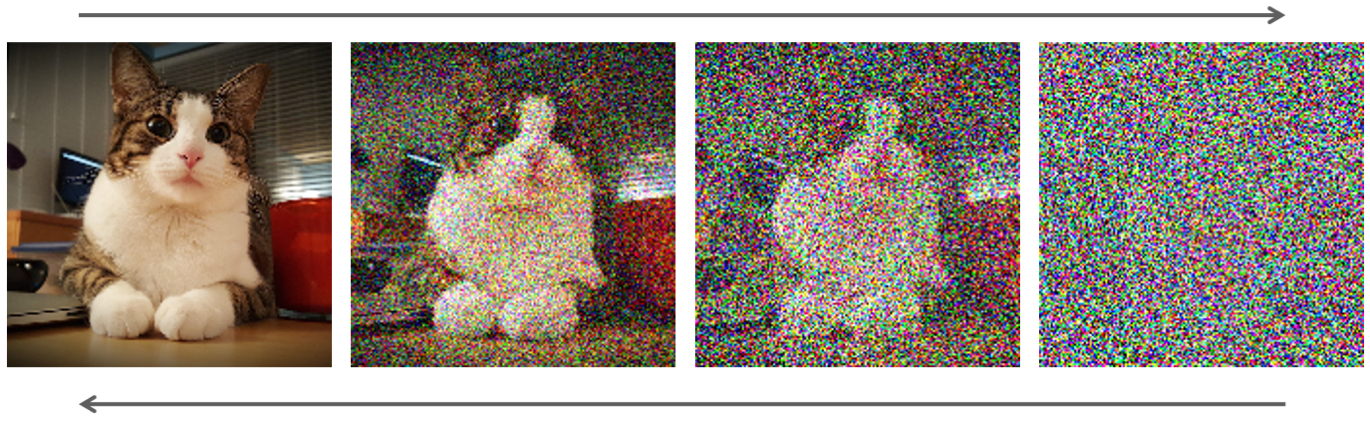
\includegraphics[width=0.9\textwidth]{figures/Diffusion_Models/Generation-with-Diffusion-Models.png}
    \caption{\cite{vahdat2022improving}}
\end{figure}
\end{frame}

\begin{frame}{Diffusion models en la actualidad}
Los diffusion models suponen la tecnología para generación de imágenes \alert{más avanzada} actualmente.

Aplicaciones como \alert{Stable Diffusion} utilizan variaciones de la arquitectura de los modelos de difusión.

Respecto a arquitecturas anteriores como las \gls{gan}, los modelos de difusión solucionan problemas como el \alert{colapso modal o gradient vanishing}, al mismo tiempo que generan imágenes \alert{más definidas y diversas}.
\end{frame}

\begin{frame}{Cadenas de Markov}
La arquitectura básica de un diffusion model se basa en las \alert{cadenas de Markov}, que es un modelo probabilístico de cambio de estados.

La principal idea es a partir de una imagen\footnote{Aunque los diffusion models se pueden aplicar a distintas fuentes de datos, por simplicidad de hablará sólo de imágenes.} generar \alert{versiones más ruidosas} de la misma de manera iterativa y encadenada.

Finalmente, una \alert{red de neuronas} aprenderá a realizar el proceso inverso, eliminar el ruido de las imágenes.

\begin{figure}
    \centering
    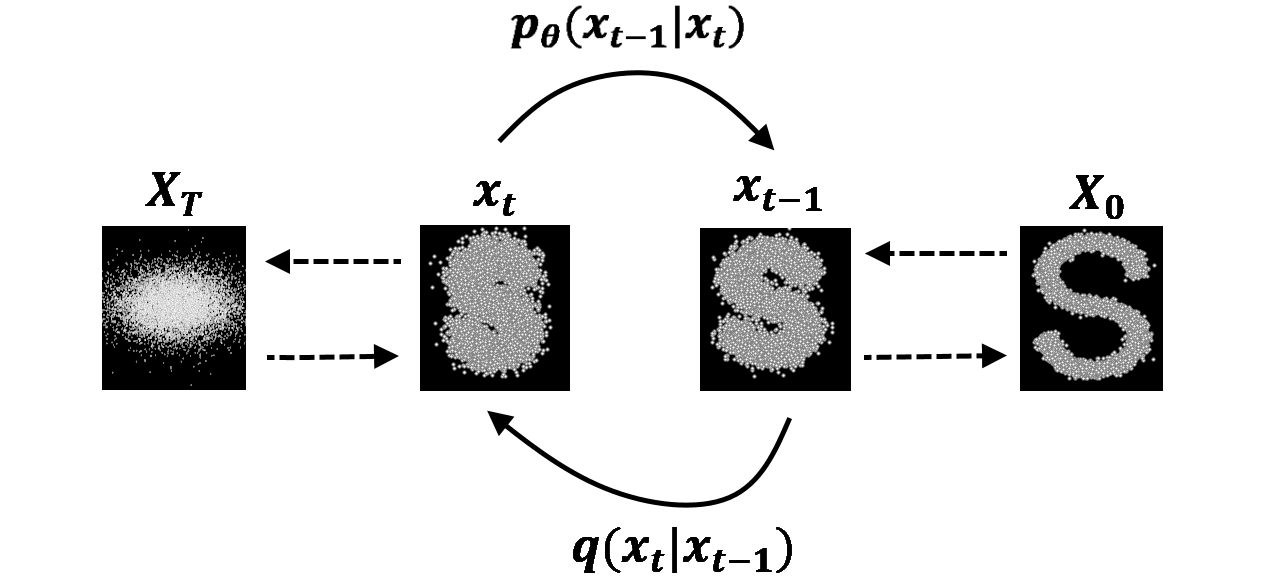
\includegraphics[width=0.6\textwidth]{figures/Diffusion_Models/DifussionModel_Basic.png}
    \caption{\cite{DifussionModel_Basic}}
\end{figure}
\end{frame}

\section{Sampleo de datos (difusión directa e inversa)}

\begin{frame}{Difusión directa}
Como se ha explicado anteriormente, el funcionamiento de los diffusion models se basa en añadir iterativamente \alert{ruido} a la imagen de entrada.

Cada instante $t+1$ es generado a partir del instante $t$ añadiendo \alert{ruido gaussiano} a la imagen.

\begin{figure}
    \centering
    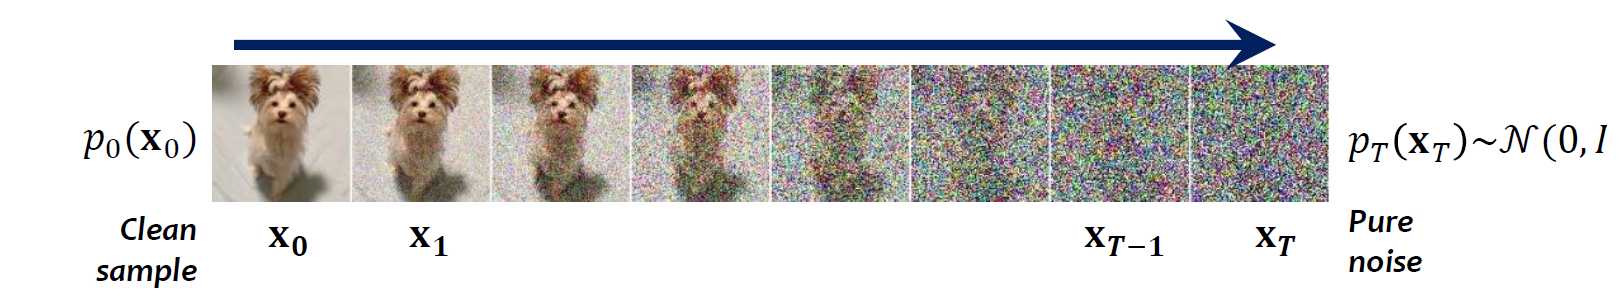
\includegraphics[width=\textwidth]{figures/Diffusion_Models/Noising_Process.png}
    \caption{\cite{vahdat2022improving}}
\end{figure}

Cabe destacar que la \alert{magnitud} del ruido generado depende el instante \alert{$t$} en el que se encuentre ese ejemplo.
\end{frame}

\begin{frame}{Difusión directa}
A través de la introducción de \alert{ruido} en las imágenes, se consigue cambiar la \alert{distribución de datos} de los ejemplos del dataset. Cada eslabón de la \alert{cadena de Markov} de nuestro modelo corresponde a una distribución distinta.

Para el instante \alert{$T$} la distribución seguida por los datos será una \alert{gaussiana}.

\begin{figure}
    \centering
    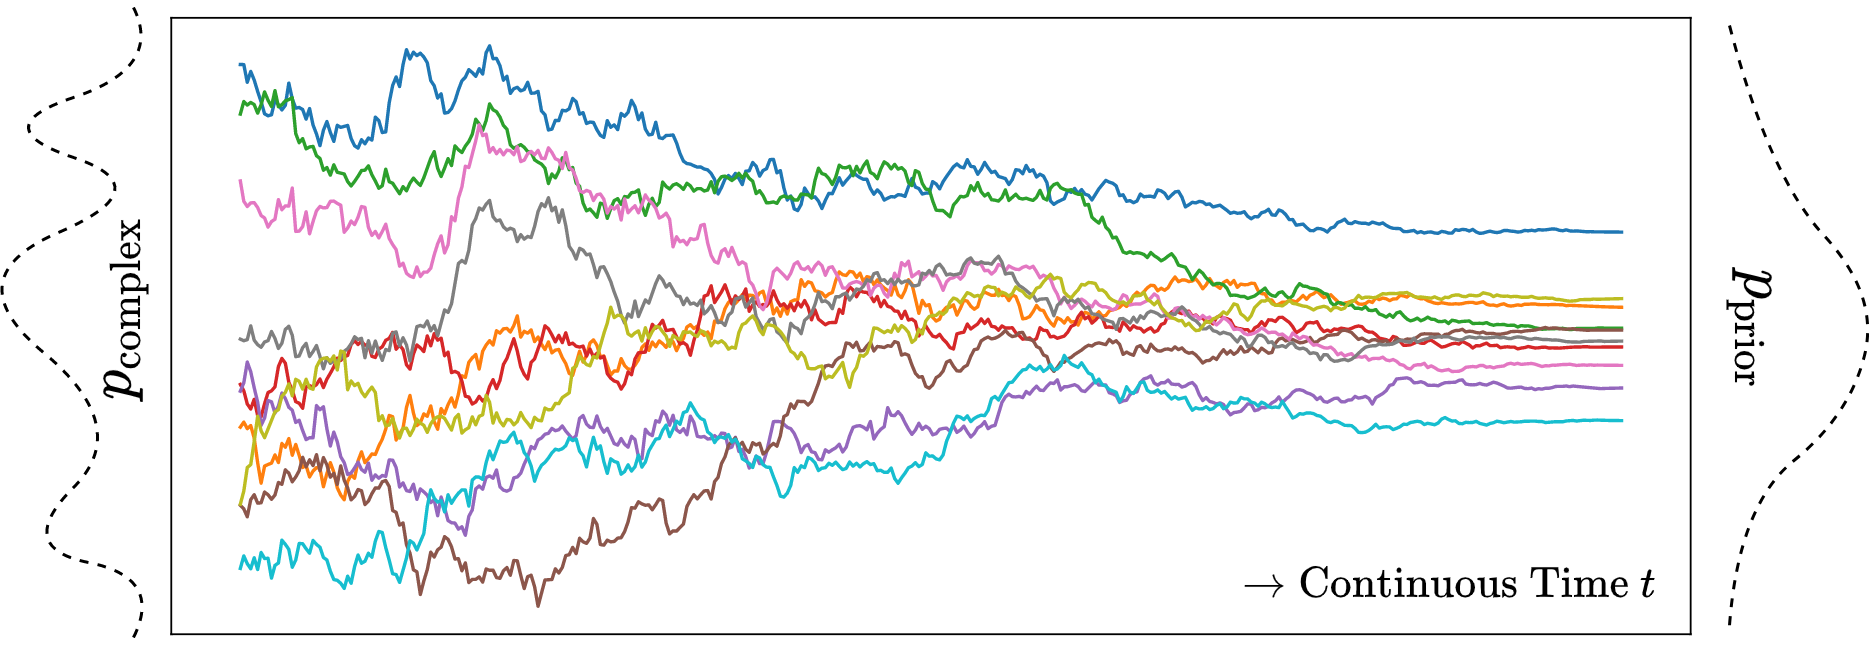
\includegraphics[width=\textwidth]{figures/Diffusion_Models/ForwardDiffusion.png}
    \caption{\cite{ForwardDiffusion}}
\end{figure}
\end{frame}

\begin{frame}{Planificador de ruido}
A la hora de introducir ruido de manera \alert{iterativa} en las imágenes que se están procesando hay distintas alternativas.

Para cada imagen generada en un instante $t$ esta se puede definir como:

\begin{equation}
    x_t = \sqrt{1-\beta_t} x_{t-1} + \sqrt{\beta_t} \epsilon_{t-1}
\end{equation}

donde $\beta$ es el \alert{diffusion rate}, que se calcula para cada instante $t$ dependiendo de un planificador llamado "\alert{variance scheduler}". Y $\epsilon_{t-1}$ es el ruido de cada instante anterior tal que \alert{$\epsilon \sim \mathcal{N}(0,1)$}.

\end{frame}

\begin{frame}{¿Por qué llegar hasta imágenes completamente ruidosas?}
La idea para generar \alert{nuevas imágenes} es generar \alert{ruido aleatorio} y realizar le difusión inversa.

De esta manera es posible generar \alert{nuevos ejemplos} aleatoriamente, ya que la distribución de datos del instante \alert{$T$} es conocida y la del instante \alert{$0$} se calcula a través del proceso de difusión inversa.
\end{frame}

\begin{frame}{Difusión inversa}
La idea del proceso de inverse diffusion es volver al \alert{ejemplo original} partiendo del \alert{ruidoso}. 

Para ello se realiza \alert{iterativamente} la operación de pasar del instante \alert{$t$} al instante \alert{$t-1$}.

Para generar la imagen del instante \alert{$t-1$} son necesarios:
\begin{itemize}
    \item La \alert{imagen de entrada} del instante \alert{t}.
    \item El \alert{ruido} de dicha imagen calculado con nuestra red de neuronas.
    \item Un algoritmo para \alert{sustraer} el ruido de la imagen.
\end{itemize}
\end{frame}

\begin{frame}{Algoritmo DDPM}
El algoritmo \gls{ddpm}, propuesto en el año 2020 \cite{ho2020denoising}, es el \alert{causante de la popularidad} que han ganado los diffusion models los últimos años.

Este algoritmo permite \alert{eliminar} el ruido de una imagen para recuperarla a su estado original.

Una de las características de \gls{ddpm} es que añade \alert{cierta cantidad de ruido} tras haberlo eliminado. Esto se hace para que la imagen de salida siga la misma \alert{distribución de datos} del instante $t$.
\end{frame}

\begin{frame}{Algoritmo DDPM}
Añadiendo cierto ruido tras cada paso de la difusión inversa, se consigue aumentar la \alert{diversidad} en las imágenes generadas, evitando el colapso modal.

\begin{figure}
    \centering
    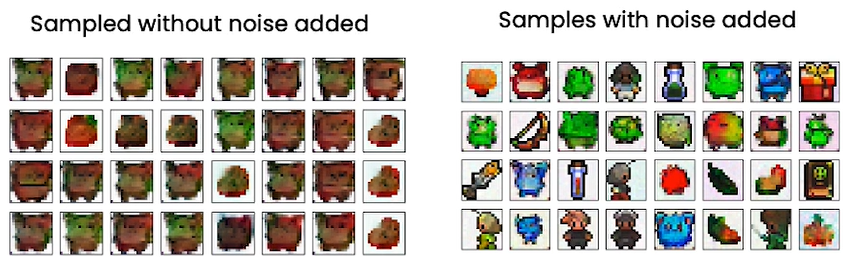
\includegraphics[width=\textwidth]{figures/Diffusion_Models/DDPM_Variation.png}
    \caption{\cite{DeepLearningDifussionModelCourse}}
\end{figure}
\end{frame}

\section{Redes neuronales y entrenamiento}

\begin{frame}{Arquitectura}
Para poder realizar el paso de \alert{inverse diffusion} utilizaremos redes neuronales, que serán capaces de calcular el \alert{ruido} de una imagen de entrada.

Dichas redes deberán calcular el \alert{ruido} presente en las imágenes que se le presenten como entrada. Para ello es necesario que la red conozca el instante \alert{$t$} en el que se encuentra.

\begin{figure}
    \centering
    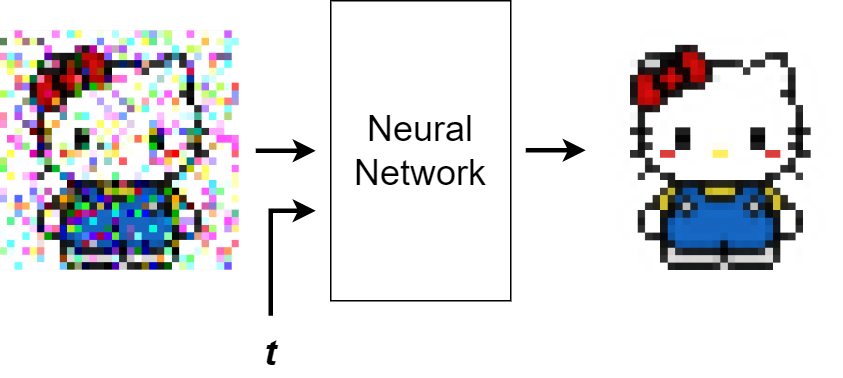
\includegraphics[width=\textwidth]{figures/Diffusion_Models/Architecture.png}
\end{figure}
\end{frame}

\begin{frame}{Autoencoder para obtener el ruido}
La solución más común para este tipo de problemas es el uso de \alert{Autoencoders}. Como se ha visto anteriormente estos modelos generan como salida datos de la misma \alert{dimensionalidad} que los de entrada.

La función del Autoencoder será obtener cuál es el \alert{ruido} de la imagen.

\begin{figure}
    \centering
    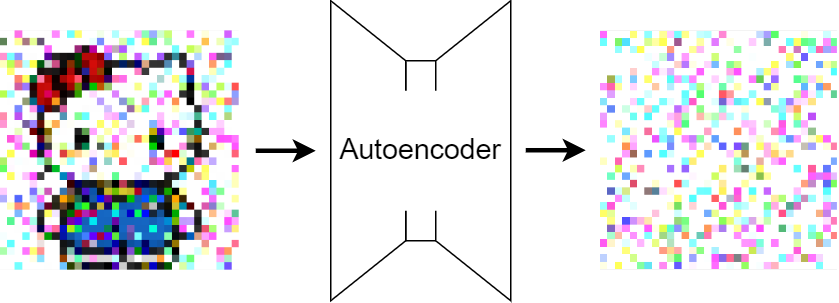
\includegraphics[width=\textwidth]{figures/Diffusion_Models/Autoencoder_Denoising.png}
\end{figure}
\end{frame}

\begin{frame}{U-Net}
La arquitectura \alert{más habitual} para los diffusion models es la U-Net, por sus propiedades a la hora de recuperar información manteniendo la \alert{definición} de las imágenes.

Aunque cabe destacar que dependiendo del \alert{conjunto de datos} que se esté utilizando esto puede cambiar. E.g. diseñar un modelo de difusión para generar música nueva.

\begin{figure}
    \centering
    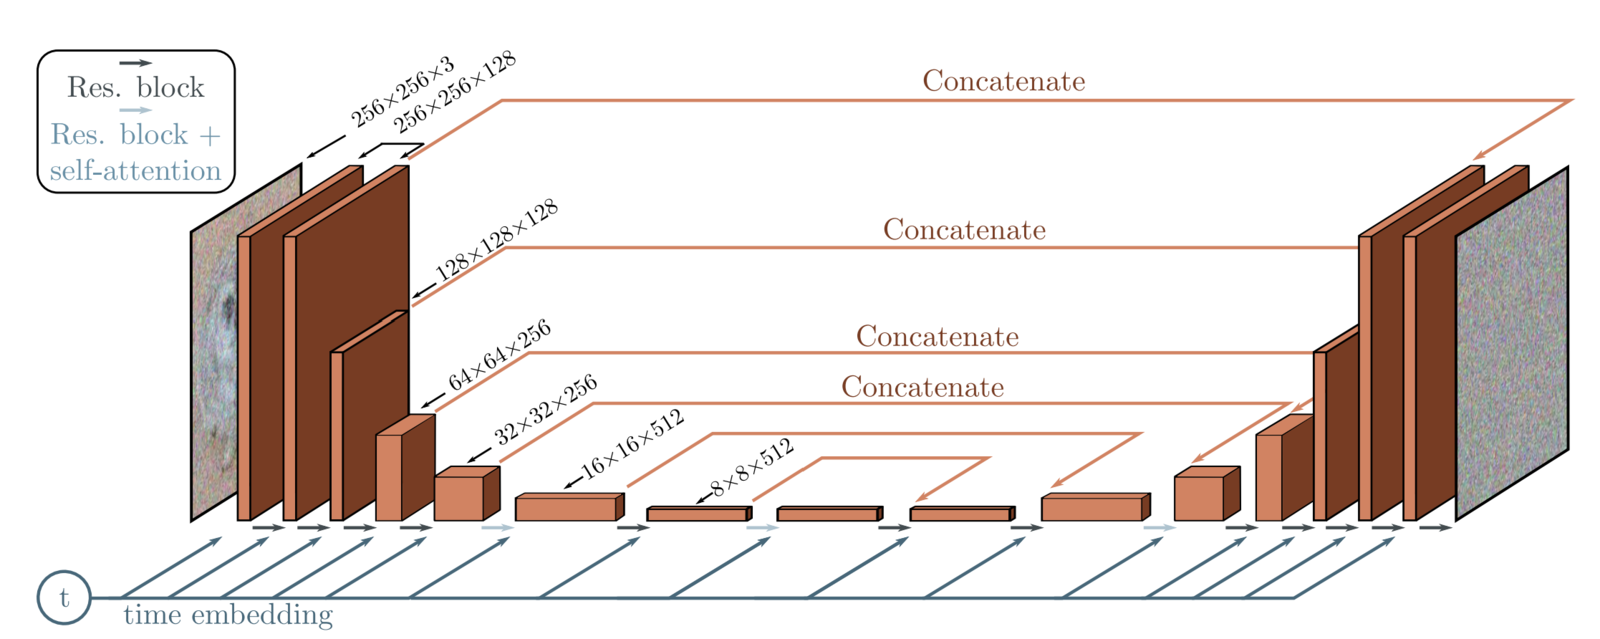
\includegraphics[width=\textwidth]{figures/Diffusion_Models/U-Net.png}
    \caption{\cite{U-Net}}
\end{figure}
\end{frame}

\section{Condicionamiento de la salida}

\begin{frame}{Cómo elegir lo que se genera}
A veces se desea tener cierto \alert{control} sobre aquello que está generando nuestro modelo. Para ello tenemos que ser capaces de añadir cierta \alert{información extra} a la red de neuronas.

Esta información extra se usará durante el \alert{entrenamiento} para condicionar a la red a aprender la \alert{distribución de datos} de las etiquetas que la condicionen.

De esta manera, cuando se quiera generar nueva información, se usará esas \alert{etiquetas} para generar lo que se quiera.
\end{frame}

\begin{frame}{Context embedding}
Esto se realiza a través del conocido como \alert{context embedding}. Este embedding se añade después de cada capa de la misma manera que el \alert{tiempo $t$}.

Una de las ventajas de los embeddings es que puedes \alert{combinar información}. Por ejemplo de la siguiente manera:

\begin{figure}
    \centering
    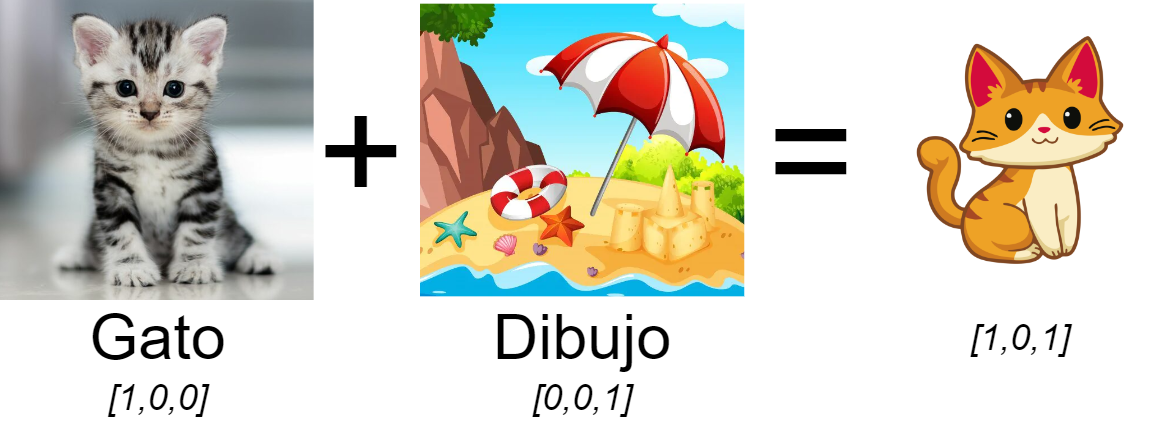
\includegraphics[width=\textwidth]{figures/Diffusion_Models/Embedding_Combination.png}
\end{figure}
\end{frame}

\begin{frame}{Context embedding}
Este embedding es \alert{alimentado} a la red después de cada bloque convolucional. De esta manera se \alert{condiciona} a la red a que aprenda el contexto de la imagen.

\begin{figure}
    \centering
    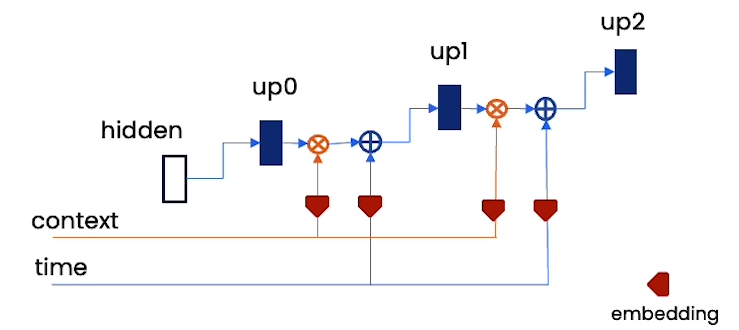
\includegraphics[width=\textwidth]{figures/Diffusion_Models/Context_Embedding.png}
    \caption{\cite{DeepLearningDifussionModelCourse}}
\end{figure}
\end{frame}

\begin{frame}{Combinando con transformers}
Si este embedding añadido se realiza con \alert{transformers}, entonces somos capaces, por ejemplo, de controlar la salida a través de texto.

Este tipo de soluciones son las que hoy en dia se utilizan en \alert{dall-e} o \alert{Stable Diffusion}.
\end{frame}

\begin{frame}{Resumen diffusion models}
\begin{figure}
    \centering
    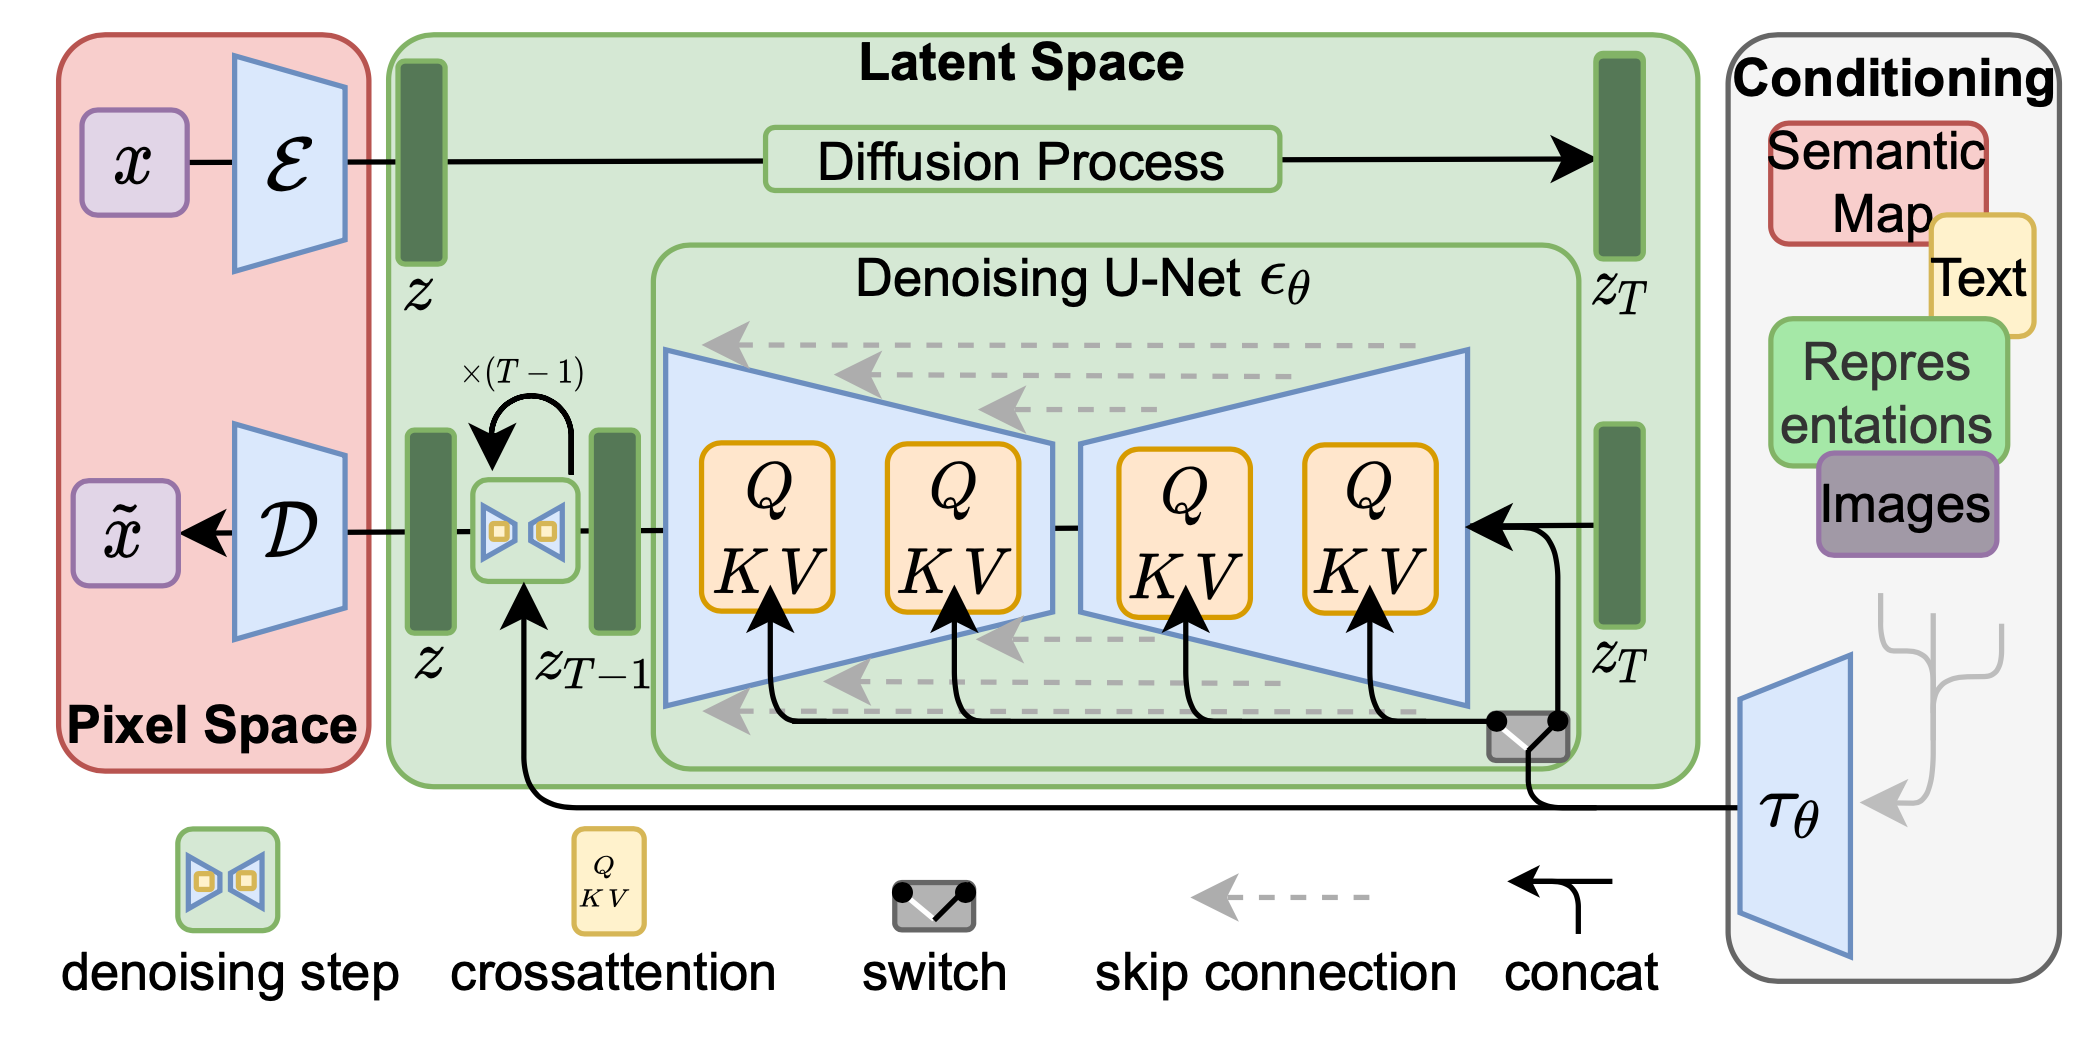
\includegraphics[width=\textwidth]{figures/Diffusion_Models/Difussion_Model.png}
    \caption{\cite{rombach2022high}}
\end{figure}
\end{frame}

\section{Mejoras en el tiempo de inferencia}

\begin{frame}{Algoritmo DDIM}
El algoritmo \gls{ddim} \cite{song2020denoising} es una alternativa a \gls{ddpm} más \alert{rápida y eficiente}.

Se basa en la idea de saltar varios pasos de la \alert{inverse difussion} de una única vez.

\begin{figure}
    \centering
    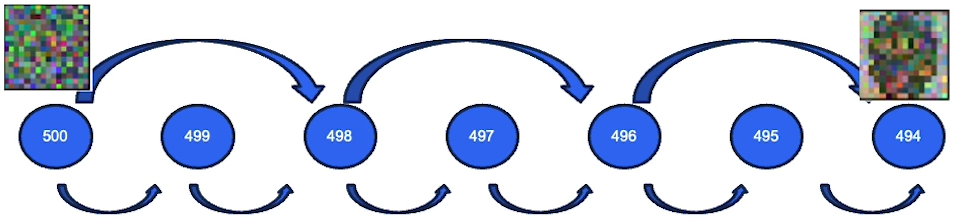
\includegraphics[width=\textwidth]{figures/Diffusion_Models/DDIM.png}
    \caption{\cite{DeepLearningDifussionModelCourse}}
\end{figure}
\end{frame}

\begin{frame}{Algoritmo DDIM}
La principal característica que permite a \gls{ddim} \alert{saltar pasos} del proceso es que no es un modelo probabilístico, si no \alert{determinista}.

De esta manera se elimina la \alert{aleatoriedad} de las cadenas de Markov.

El algoritmo \gls{ddim} llega a ser \alert{10 veces} más eficiente que el \gls{ddpm}.
\end{frame}

\section{Ejemplos y aplicaciones}

\begin{frame}{Generación de imágenes}
Quizás las aplicaciones más conocidas de los \alert{diffusion models} son \alert{Stable Diffusion} o \alert{Dall-e 2}.

\begin{figure}
    \centering
    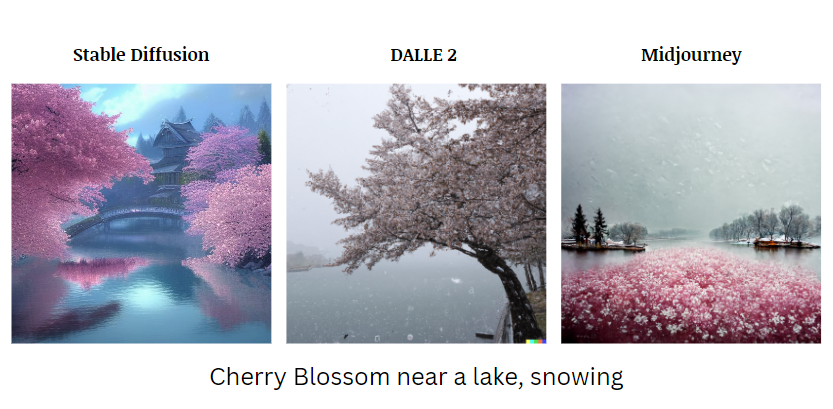
\includegraphics[width=0.8\textwidth]{figures/Diffusion_Models/Stable_Diffusion_Dalle.png}
    \caption{\cite{SD_vs_DE_vs_MJ}}
\end{figure}

Stable Diffusion utiliza una architectura llamada \alert{\gls{ldm}}. Por su parte tanto Midjourney como Dall-e 2 usan tecnologías propietario desconocidas.
\end{frame}

\begin{frame}{\acrlong{ldm}}
La arquitectura \gls{ldm} \cite{rombach2022high} se basa en \alert{comprimir la información} en un espacio latente para realizar con este el proceso de difusión.

De esta manera la \alert{dimensión} de la información tratada se reduce drásticamente. Con ello se permiten mejorar los tiempos de inferencia y entrenamiento.
\end{frame}

\begin{frame}{Generación de video: Align your latents}
A parte de generar imágenes, existen alternativas capaces de generar vídeo. Uno de los trabajos más importantes fue publicado por Andreas Blattmann et al., de NVIDIA \cite{blattmann2023align} en el año 2023.

Este trabajo usa la arquitectura \gls{ldm} introduciendo un \alert{batch de imágenes} que corresponden con un vídeo de 4,7 segundos.

\begin{figure}
    \centering
    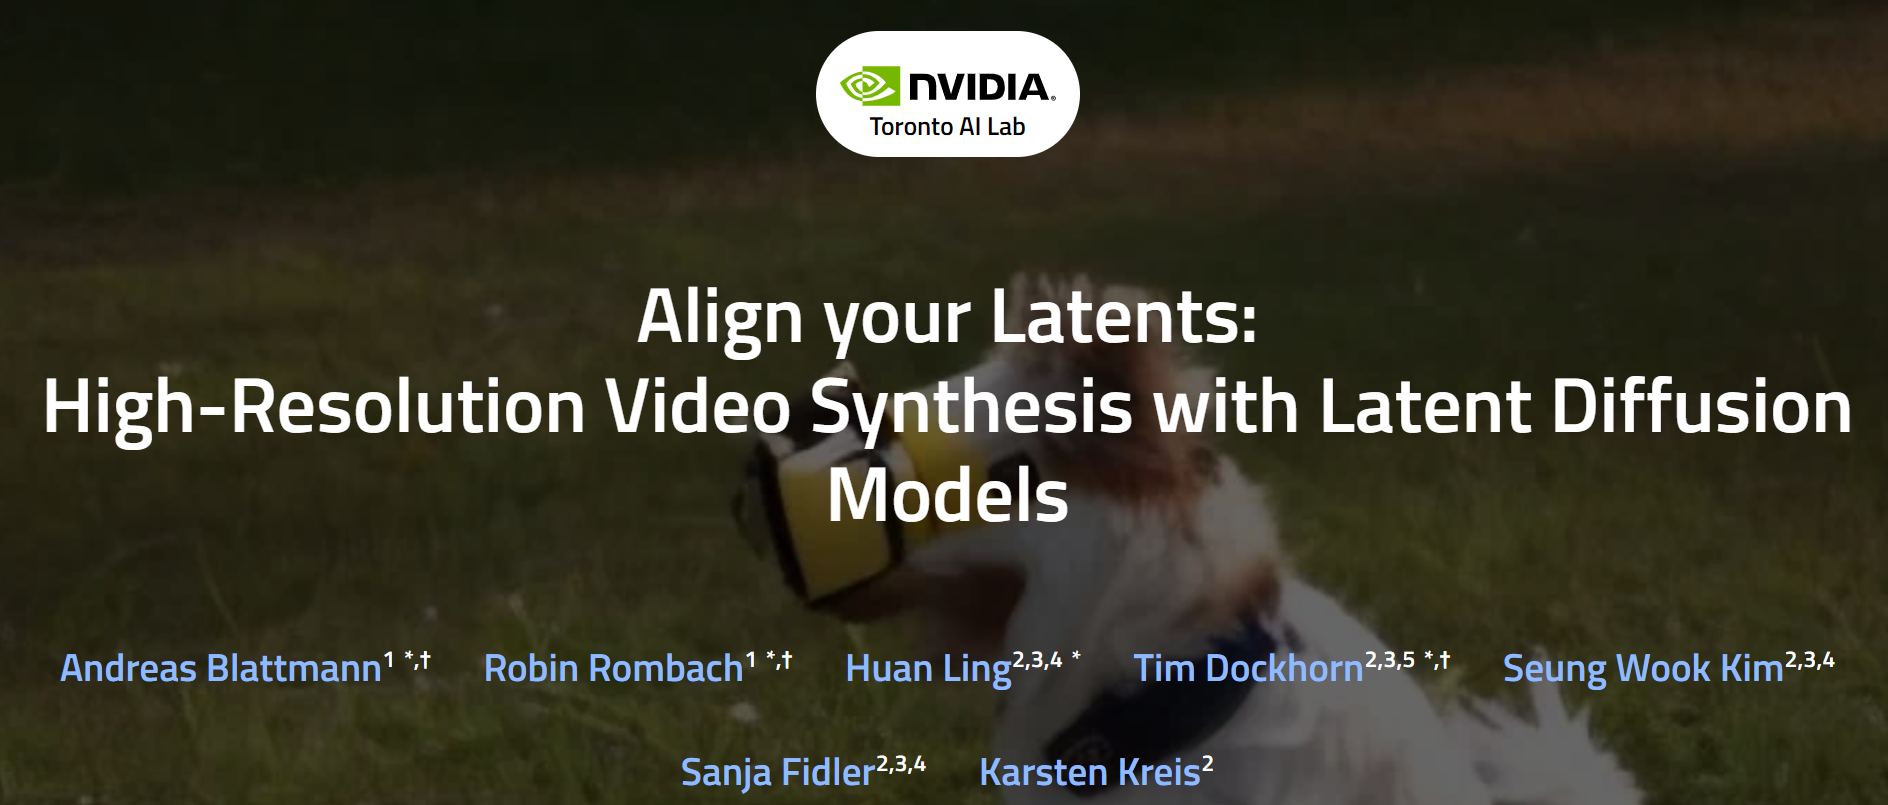
\includegraphics[width=0.8\textwidth]{figures/Diffusion_Models/AlignYourLatent_NVIDIA.png}
    \caption{Ejemplos del resultado en la \href{https://research.nvidia.com/labs/toronto-ai/VideoLDM/samples.html}{\alert{Web de NVIDIA}}}
\end{figure}
\end{frame}

\begin{frame}{Align your latents}
En la arquitectura propuesta se usan ideas también de \gls{gan}, como el uso de un \alert{discriminador} para que los videos mantengan fotorealismo.

\begin{figure}
    \centering
    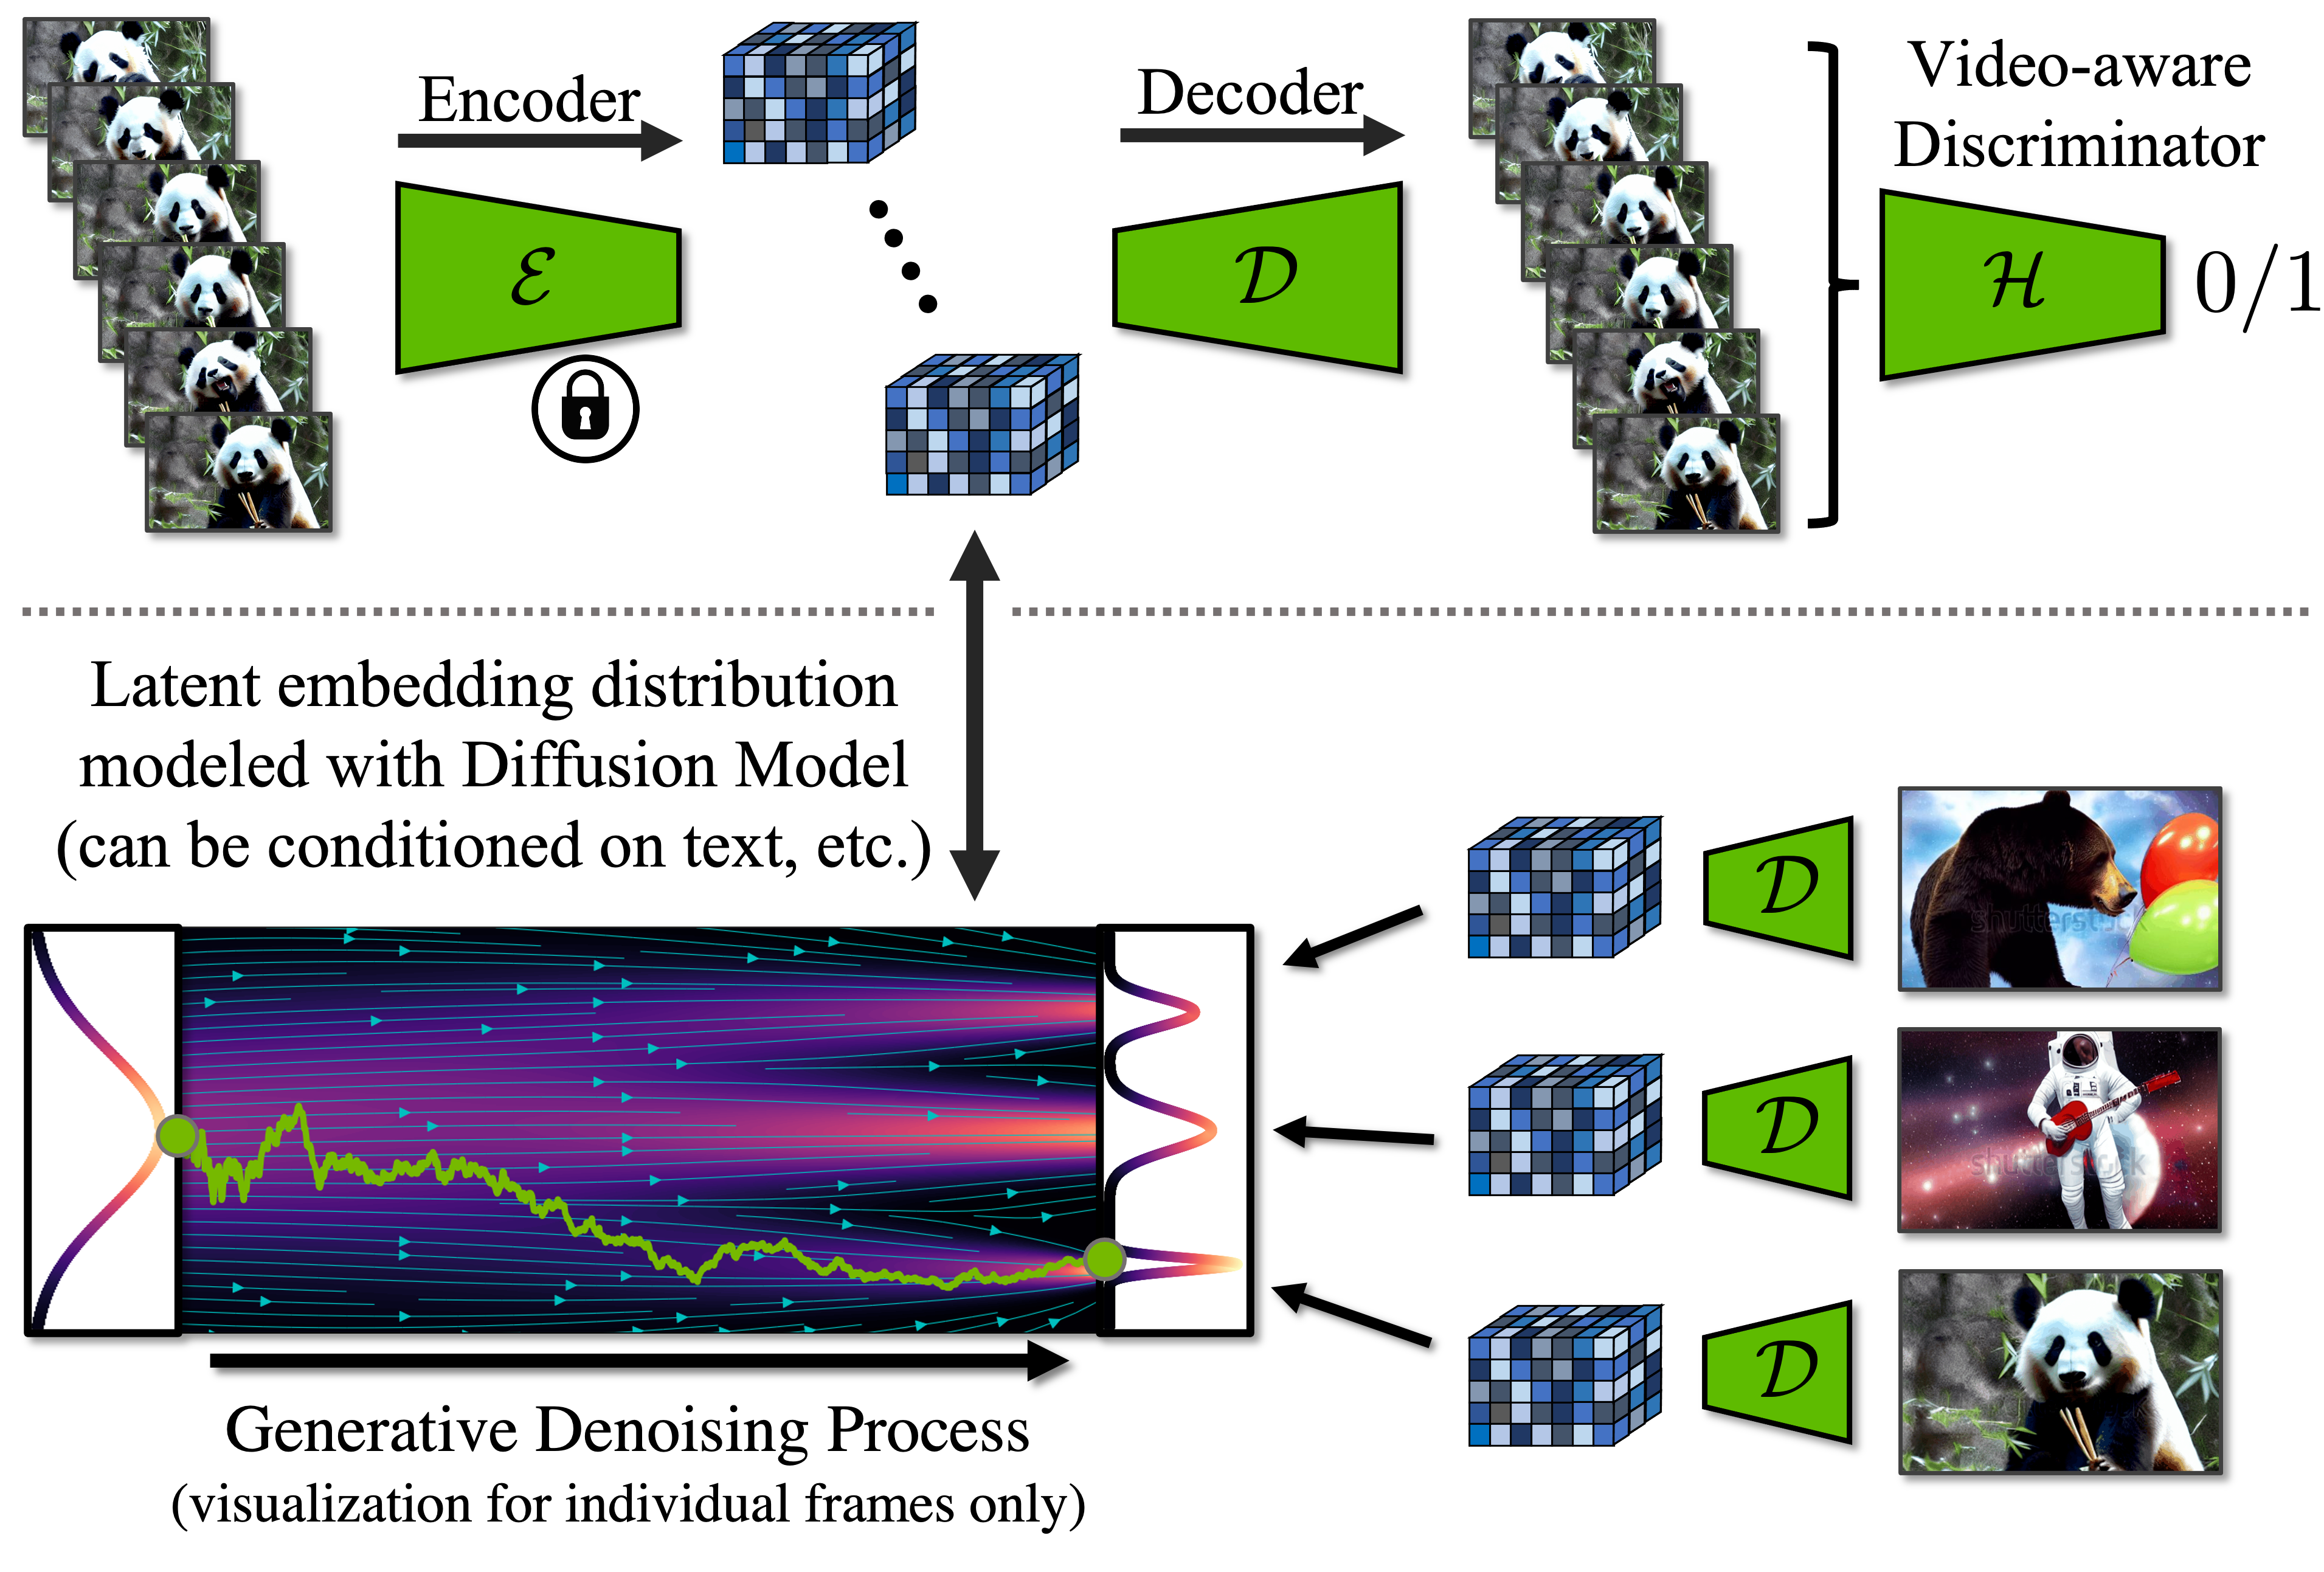
\includegraphics[width=0.8\textwidth]{figures/Diffusion_Models/AlignYourLatent.png}
    \caption{\cite{blattmann2023align}}
\end{figure}
\end{frame}

\begin{frame}{Generación de música: Noise2Music}
El trabajo de \alert{Noise2Music} \cite{huang2023noise2music} propone el uso de modelos de difusión para \alert{generar música} a partir de un \alert{texto}.

Para ello se proponen 2 componentes principales:

\begin{itemize}
    \item El \alert{diffusion generator} se encarga de generar la \alert{base de la música} a baja calidad a partir de la \alert{query de texto}.
    \item Una serie de \alert{diffusion cascader} que se encargan de mejorar la \alert{calidad} iterativamente.
\end{itemize}

\begin{figure}
    \centering
    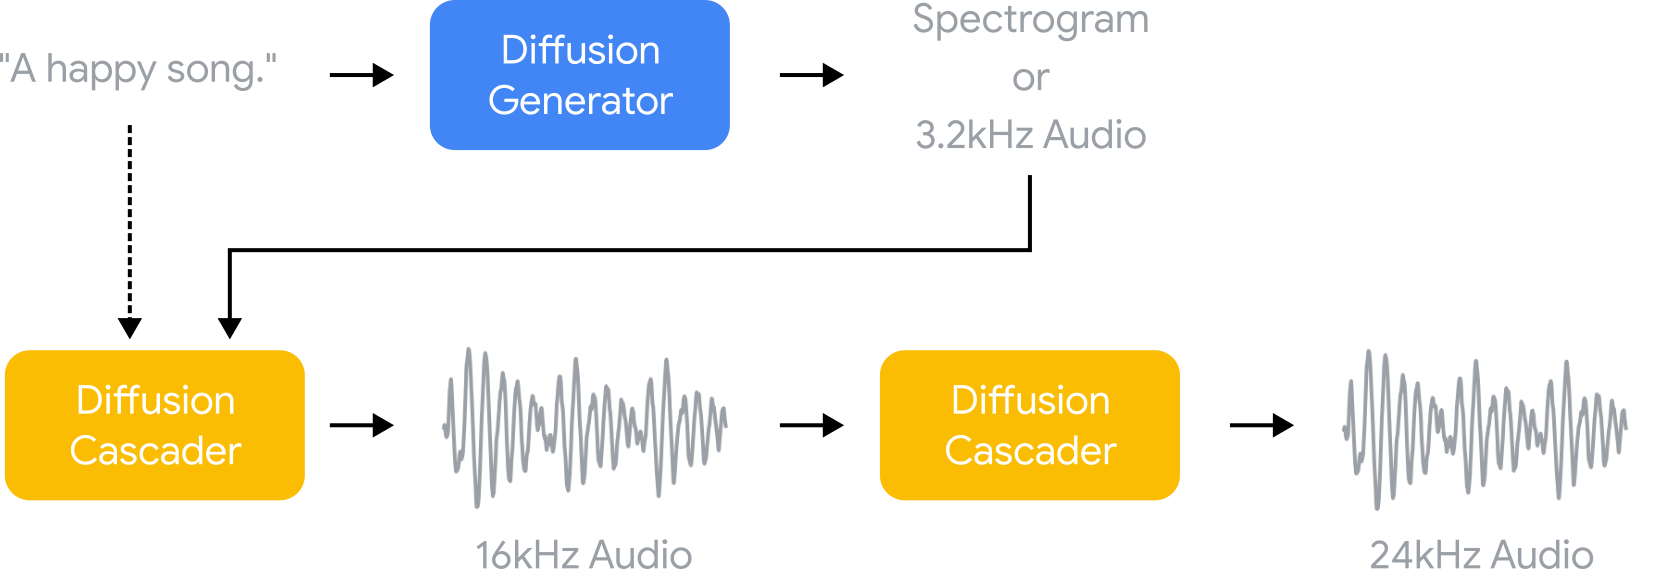
\includegraphics[width=0.8\textwidth]{figures/Diffusion_Models/Noise2Music.png}
    \caption{\cite{huang2023noise2music}}
\end{figure}
\end{frame}

\begin{frame}{Noise2Music}
En el trabajo original proponen dos alternativas para tratar el audio:
\begin{itemize}
    \item \alert{Ondas sonoras}: Tratan la música como una serie temporal. Para ello se usa 
    una \alert{1D U-Net} en la que las convoluciones observan una única dimensión.
    
    \item \alert{Espectrograma}: Una alternativa bastante común para tratar con audio es transformarlo a imagen usando su \alert{espectograma}.
\end{itemize}
\end{frame}

\addcontentsline{toc}{section}{Referencias}

\begin{frame}[allowframebreaks]{Referencias}
    \bibliographystyle{unsrt}
    \bibliography{Slides/references.bib}
\end{frame}

\begin{frame}{Contribuciones de las diapositivas}
\begin{itemize}
    \item \textbf{Autor original de las diapositivas:} Guillermo Iglesias Hernández
    \item Diapositivas basadas en el curso: \textit{How Diffusion Models Work}, de Sharon Zhou. \url{https://learn.deeplearning.ai/diffusion-models} \cite{DeepLearningDifussionModelCourse}.
\end{itemize}
\end{frame}

\end{document}